\documentclass[12pt]{article}
\usepackage[a4paper, margin=.30in]{geometry}
\usepackage{graphicx ,
            wrapfig,
            xcolor, 
            enumerate,
            amsmath,fontenc,tcolorbox
            }
\usepackage[european, straightvoltages,EFvoltages]{circuitikz}
\newcommand\headerMe[2]{\noindent{}#1\hfill#2}
\renewcommand{\thesection}{\Roman{section}}

\title{Leçon : }
\author{Zakaria HAOUZAN}
\date{\today}

\begin{document}
% headers --------------
\headerMe{Matière : Physique-Chimie}{Professeur : Zakaria HAOUZAN}\\
\headerMe{Unité : La Mécanique}{Établissement : Lycée SKHOR qualifiant}\\
\headerMe{Niveau : TCS}{Heure : 3H}\\

% ------Content ________
\begin{center}
    \Large{Leçon $N^{\circ}9$: \color{red}La Tension électrique}
\end{center}

\section{Situation-problème}
Tous les appareils et les composants électriques qui nous entourent, fonctionnent avec une
tension électrique.
\\Qu’est-ce qu’une tension électrique ?
\\ Et comment peut-on la mesurer?

\section{Notion de tension électrique:}
\subsection{Définition:}
La tension électrique $U_{AB}$ entre ces deux points A et B d'un circuit électrique est la différence de potentiel entre ces deux points (son unité est le volt (V) ).
$$U_{AB} = V_A - V_B$$

$V_B$ : potentiel électrique au point B \hspace{1cm} $V_A$ : potentiel électrique au point A

Remarque: le potentiel électrique n'est pas directement mesurable. Il définit l'état électrique d'un point de l'espace. (il s'exprime en en Volt).

\subsection{La tension grandeur algébrique mesurable:}
\begin{itemize}
    \item Si $V_A$ > $V_B$ , $V_A - V_B > 0$ , donc $U_{AB} > 0$
    \item Si $V_A$ < $V_B$ , $V_A - V_B < 0$ , donc $U_{AB} < 0$
    \item Si $V_A$ = $V_B$ , $V_A - V_B = 0$ , donc $U_{AB} = 0$
\end{itemize}
\subsection{Représentation de la tension électrique}
La tension électrique UAB est représentée par une flèche dirigée du point B vers le point A . 
  \begin{center}
  \begin{circuitikz}[european resistors]
      \draw (-0.5,0.1)node{A} (0,0)to[R,v<=$U_AB$,i=I, name=R] (2,0);
      \draw (2.2, 0) node{B};
    
  \end{circuitikz}
  \end{center}

\begin{wrapfigure}[4]{r}{0.39\textwidth}
    \vspace{-1cm}
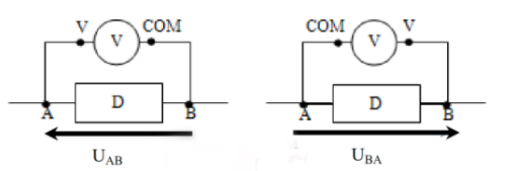
\includegraphics[width=0.39\textwidth]{./img/img_voltage_mesure_00.png}
\end{wrapfigure}
\section{Mesure de la tension électrique:}
\subsection{Appareils de mesure de la tension électrique:}
On peut mesurer la tension électrique :
\\-à l'aide d'un voltmètre( à aiguille ou numérique)
\\-ou bien à l'aide d'un oscilloscope.
\\Pour mesurer la tension électrique entre deux points le voltmètre doit être monté en derivation( en parallèle) entre
ces deux points.

\subsection{Voltmètre à aiguille : }
La tension mesurée est donné par la relation suivante : 
$$U=\frac{c.n}{n_0}$$

c : le Calibre utilisé
\\n : nombre de divisions ( de graduations ) indiqué par l’aiguille
\\$n_0$ : nombre de graduations total du cadran (de l’échelle de lecture)

La mesure de la tension électrique est accompagnée avec une
incertitude absolue $\Delta{U}$ provoquée par l’appareil , il est déterminé par la
relation suivante : $\Delta{U} = \frac{c.a}{100}$

a : la classe de l’appareil. Elle est donnée par le fabriquant dans un coin de l’appareil

\begin{tcolorbox}{Remarque : }
- U dépend de c et a
\\- Si a la classe de l’appareil est plus petite, alors l’appareil est plus précis ;
\\- Si le calibre C est plus petit alors l’incertitude absolue I est plus petite donc l’appareil est plus précis , c’est pourquoi on choisit le calibre le plus petit pendant la mesure de la tension électrique

    Incertitude relative : $\frac{\Delta{U}}{U}$ représente la précision de mesure de cet appareil elle s’exprime généralement en pourcentage \% .
\end{tcolorbox}

\subsection{Mesure de la tension électrique grâce à un oscilloscope : }
L'oscilloscope est un appareil électrique permettant de visualiser et de mesurer le tension électrique entre
les bornes d’un dipôle dans un circuit.

\begin{center}
  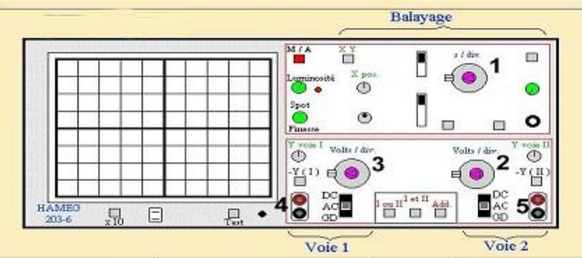
\includegraphics[width=0.75\textwidth]{./img/img_oscilloscope_01.png}


\end{center}
\begin{wrapfigure}[7]{r}{0.5\textwidth}
    \vspace{-1cm}
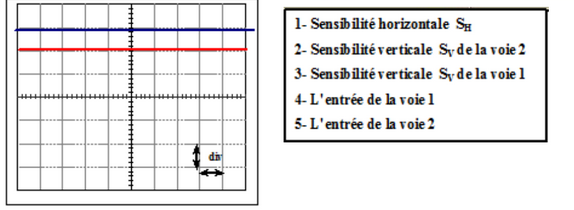
\includegraphics[width=0.5\textwidth]{./img/img_tension_u_02.png}
\end{wrapfigure}

Pour mesurer la tension entre les bornes d’un générateur, on branche la borne positive du générateur à
l’entrée $Y_1$ de la voie N°1 de l’oscilloscope et la borne négative à la masse , on obtient un trait lumineux
horizontal déplacé vers le haut par nombre $Y$ de divisions . En connaissant la valeur de la sensibilité
verticale exprimé en $V / div$ , la tension entre les bornes du générateur est $U = y . S_v$ 
\\avec :
$S_v$ : la sensibilité verticale


\begin{center}
  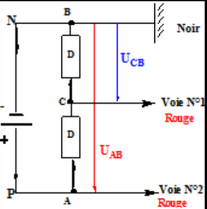
\includegraphics[width=0.175\textwidth]{./img/img_circuit_03.png}
\end{center}
Données :
Sensibilité verticale SV de l’entrée Y1 : $S_V = 1 V / div$
Sensibilité verticale SV de l’entrée Y2 : $S'_V = 2 V / div$

Calculer la tension $U_{CB}$ et $ U_{AB}$

\section{Propriétés de la tension électrique : }

\begin{wrapfigure}[6]{r}{0.39\textwidth}

    \vspace{-1.5cm}
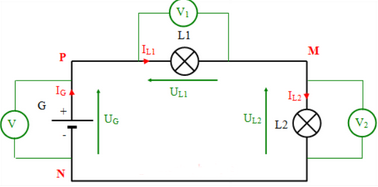
\includegraphics[width=0.39\textwidth]{./img/img_circuit_serie_04.png}
\end{wrapfigure}


\subsection{La tension électrique dans un circuit en série : Loi de l’additivité des tensions}
On réalise le circuit en série suivant, composé de : Générateur G , Lampe 1 , Lampe 2 , et trois voltmètres.
On mesure la tension électrique aux bornes de chaque dipôle,on obtient :
$U_{MN} = 4,5 V$ , $U_{PM} = 7,5 V$ , $U_{PN} = 12 V$

Etude pratique : $U_{MN} = 4,5 V$ , $U_{PM} = 7,5 V$ , $U_{PN} = 12 V$ on constate que $U_{PN} = U_{PN} + U_{MN}$

Etude théorique :
$U_{PN}=V_P - V_N = V_P - V_N + V_M - V_M = ( V_P - V_M ) + ( V_M - V_N )$
Donc $U_{PN} = U_{PN} + U_{MN}$
C’est la loi d’additivité des tensions

\begin{tcolorbox}
Conclusion : La loi d’additivité des tensions
Dans un circuit en série , la tension électrique UAB est la somme de toutes les tensions entre les bornes des
dipôles montés en série entre les deux points A et B
\end{tcolorbox}



\begin{wrapfigure}[6]{r}{0.39\textwidth}

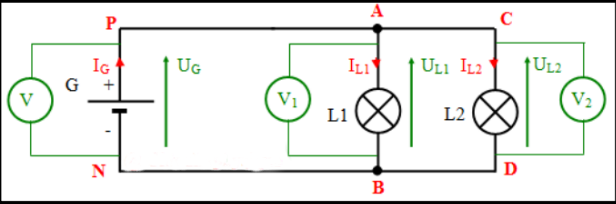
\includegraphics[width=0.39\textwidth]{./img/img_circuit_para_05.png}
\end{wrapfigure}


\subsection{La tension électrique dans un circuit en parallèle : l’unicité de la tension}
On réalise le circuit électrique en parallèle suivant, composé de : Générateur G , Lampe 1 , Lampe 2 , et trois
voltmètres. On mesure la tension électrique électrique
dans les différentes branches du circuit et on obtient :
$U_{PN} = 6,0 V$ , $U_{AB} = 6,0 V$ ,$ U_{CD}= 6,0 V$

Etude pratique : $U_{PN} = 6,0 V$ , $U_{AB} = 6,0 V$ , $U_{CD}= 6,0 V$
on constate que UAB = UCD = UPN

Etude théorique :
\\$U_{PN} = V_P - V_N$
\\$U_{AB} = V_A - V_B$
\\$U_{CD} = V_C - V_D$ Or $V_P = V_A = V_c$ et $V_N = V_B = V_D$ alors $V_P - V_N = V_A - V_B = V_C - V_D$ d’où UAB=UCD=UPN C’est l’unicité de la tension

\begin{tcolorbox}
  Conclusion : l’nicité de la tension
Les tensions aux bornes de dipôles montés en dérivation (en parallèle) sont égales : UAB = UCD = UPN
\end{tcolorbox}

\section{Tension variable : }
\subsection{définition : }
Une tension est dite variable si elle prend différentes valeurs au cours du temps (  si sa valeur change avecle temps ) .

La tension est périodique lorsqu’elle se reproduit de manière identique sur des intervalles de temps
réguliers.( / lorsqu’elle est répétée de manière similaire et régulière sur des périodes du temps successives
et égales )

\subsection{Exemples des tensions variables}

\begin{center}
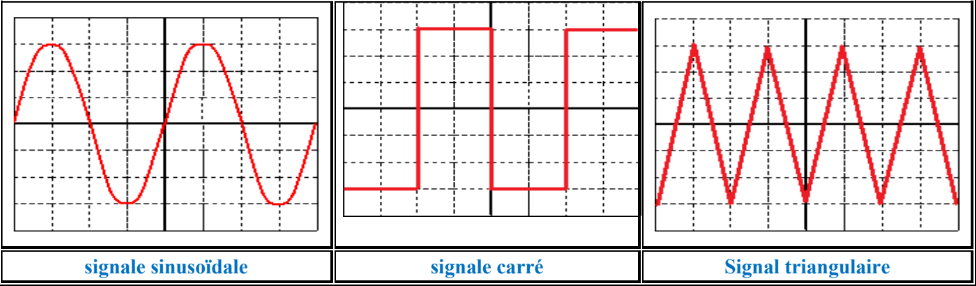
\includegraphics[width=1\textwidth]{./img/img_signal_types_06.png}
\end{center}

\begin{wrapfigure}[9]{r}{0.2\textwidth}
    \vspace{-1cm}
\includegraphics[width=0.2\textwidth]{./img/img_u_eff_sin_07.png}
\end{wrapfigure}


\subsection{Caractéristiques d’une tension alternative périodique : }
La tension alternative périodique se caractérise par des grandeurs physiques
suivantes : L’amplitude Um , la période T ou la fréquence f

\begin{itemize}
  \item Amplitude ou tension maximale Umax
On appelle amplitude, notée Umax, la valeur maximale de la tension. Elle
représente la distance entre l’axe des abscisses et un des sommets ou des
minimums.
Umax = (nombre de carreaux verticaux) x (sensibilité verticale)

\item Tension efficace Ueff :
Un oscilloscope mesure Umax et permet de voir la forme du signal électrique
Contrairement le voltmètre mesure une valeur dit La tension efficace Ueff .
    Umax / Ueff est pratiquement constant et égale à $1,414=\sqrt(2)$
    Alors $U_{eff} = \frac{U_{max}}{\sqrt(2)}$
\end{itemize}




\subsection{Période T et fréquence f : }
\begin{itemize}
  \item La période T : c’est le plus petit intervalle de temps au bout duquel la tension se reproduit ( se répète ). identiquement à elle-même . On la note T s’exprime en S

  \item La fréquence F : c’est le nombre des périodes en unité de temps ( par
seconde ) .
\end{itemize}
Pratiquement , la fréquence c’est l’inverse de la période. Elle s’exprime
en Hertz de symbole ( Hz ) : $F = \frac{1}{T}$
\\Exemple :
\\Calculer : Umax, Ueff et f
\\Données :Sensibilité horizontale SH ou vitesse de balayage : SH = 0,2 ms / div
\\Sensibilité verticale SV : SV = 2 V / div
\begin{center}
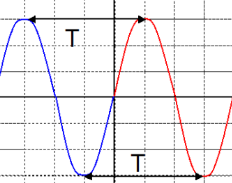
\includegraphics[width=0.4\textwidth]{./img/img_perod_08.png}
\end{center}





\end{document}
